\documentclass[12pt,a4paper]{report}

% Packages
\usepackage{graphicx}
\usepackage{amsmath}
\usepackage{hyperref}
\usepackage[german]{babel}
\usepackage{csquotes}
\usepackage{setspace}
\usepackage{titlesec}
\usepackage{tabularx}
\usepackage{booktabs}
\usepackage{array} % for 'm' column type
\usepackage{longtable}
\usepackage{anyfontsize}
\usepackage{xurl}
\usepackage[
backend=biber,
citestyle=authortitle,
bibstyle=mla
]{biblatex}
\DeclareLanguageMapping{german}{german}
\addbibresource{references.bib}
\usepackage{etoolbox}
\makeatletter
\patchcmd{\chapter}{\if@openright\cleardoublepage\else\clearpage\fi}{}{}{}
\makeatother
\makeatletter
\renewcommand{\@makechapterhead}[1]{%
\vspace*{50 pt}%
{\setlength{\parindent}{0pt} \raggedright \normalfont
\bfseries\Huge
\ifnum \value{secnumdepth}>1 
   \if@mainmatter\thechapter.\ \fi%
\fi
#1\par\nobreak\vspace{40 pt}}}
\makeatother

% newline after paragraph
\newcommand{\myparagraph}[1]{\paragraph{#1}\mbox{}\\}

% Begin Document
\begin{document}

% Title Page
\makeatletter
\begin{titlepage}
    \centering
    \vspace*{1cm}
       { 
\includegraphics[width=6cm]{img/kanti-baden.png}}\\[1cm]

    {\LARGE \textbf{Kanti Koala}}\\
    {\textbf{Die Lern- und Studienhilfsapp für Schüler:innen der Kantonsschule Baden}}\\[1cm]

    {Maturitätsarbeit, Kantonsschule Baden}\\[1cm]
    
    \textbf{Erstbetreuer: }{Michael Schneider}\\
    \textbf{Zweitbetreuerin: }{Julia Smits}\\[1cm]
    
    \textbf{Geschrieben von: }{Aryan Anand (G22b), Simon Haddon (G22b)}\\[1cm]
    \date{\large Datum: 11. November 2025}
    {\@date\\}
\end{titlepage}
\makeatother

\chapter*{Abstract}
\addcontentsline{toc}{chapter}{Abstract}
Die Kanti Koala App ist eine Webanwendung, die entwickelt wurde, um Schüler:innen der Kantonsschule Baden bei der Bewältigung ihres anspruchsvollen Schulalltags zu unterstützen. Die App bietet eine zentrale, leicht verständliche Agenda zur Organisation aller Termine, Hausaufgaben und Prüfungen. Kernstück ist ein intelligenter Lernalgorithmus, der auf Basis individueller Prioritäten und gesetzter Fristen automatisch flexible Lernblöcke in den Kalender einplant. Darüber hinaus verfügt die App über ein Notenmanagement-System zur transparenten Leistungsüberwachung und liefert zusätzliche Lerntipps und Hilfestellungen. Technisch basiert Kanti Koala auf Python/Flask und einer SQLite-Datenbank und wurde mit Fokus auf Benutzerfreundlichkeit und Datenintegrität konzipiert. Ziel ist es, den Schüler:innen zu helfen, den Überblick zu behalten, Stress zu reduzieren und das Selbstmanagement zu verbessern.

% Table of Contents
\tableofcontents

% ------------------------------Einleitung------------------------------
\chapter{Einleitung – Unsere Vision}
In der Kantonsschule Baden hat man meist viel zu tun. Es gibt nicht nur viele Prüfungen, auf die man sich vorbereiten muss, sondern auch Hausaufgaben, welche gemacht werden müssen. Wenn man alles, was man für die Schule tun muss, mit den Aktivitäten, die man in der Freizeit macht, kombiniert, merkt man, dass man viel zu tun hat. Es ist nicht leicht, das alles allein und ohne Hilfe zu bewältigen.

Deshalb haben wir uns entschlossen, eine App zu entwickeln, mit der man den Überblick über all diese Aktivitäten behalten kann. Sie organisiert sie nicht nur für die Studierenden, sondern zeigt auch an, wenn man mit etwas Bestimmtem in Verzug gerät. Diese App gibt auch Tipps, wie man effizienter lernen kann, und sie gibt sogar allgemeine Tipps über die Schule, was besonders hilfreich ist, wenn man ein:e neue:r Schüler:in ist. Generell hat die App viele Funktionen, die den Schüler:innen den Alltag erleichtern sollen.

% ------------------------------Recherche------------------------------
\chapter{Recherche}
\section{Warum brauchen wir eine Recherche?}
Da wir eine Web-App erstellen wollen, welche möglichst gut an die Bedürfnisse von Schüler:innen angepasst ist, durften wir uns nicht nur auf unsere eigenen Erfahrungen als Schüler verlassen, sondern mussten auch ein gewisses Mass an Recherche erledigen, damit wir wichtige Entscheidungen sinnvoll begründen konnten. Zu diesem Ende haben wir uns entschieden, uns tiefgründig mit unserem Zielpublikum - Schüler:innen der Kantonsschule Baden - auseinanderzusetzen, indem wir Interviews mit PPP-Lehrpersonen führten und eine Umfrage für Schüler:innen gestalteten.

Somit präsentiert sich die Recherche als einen wichtigen und umfassenden Bestandteil für die Entwicklung unserer Web-Applikation, da sie uns hilft, uns in unsere Zielgrupe zu versetzen und ihre Bedürfnisse besser zu verstehen, damit wir sie bestmöglich umsetzen können.

\section{Literaturstudie}
\subsection{Vorgehensweise}
Als erstes führten wir eine einfache und relativ oberflächliche Literaturstudie durch.
Diese Literaturstudie diente vor allem dazu, uns einen ersten Einblick in die Thematik des Lernens ausserhalb unserer eigenen Schulerfahrung zu verschaffen, damit wir uns auf einer sinnvollen Weise auf die Interviews und die Umfrage vorbereiten konnten und somit bereits früh erste informierte Entscheidungen treffen konnten, wie beispielsweise wie wir den Interviewfragebogen gestalten wollten.

Zu diesem Zweck liehen wir die folgenden zwei Bücher aus der Mediothek der Kanti Baden aus, welche uns einen differenzierten Standpunkt geben sollten:
\begin{list}{}
    \item \textbf{Buch 1}
    \item \textbf{Buch 2}
    
\end{list}
\subsection{Book 1}

\subsection{Book 2}
\section{Interviews}

\section{Umfrage}
% ------------------------------Programmieren------------------------------
\chapter{Programmieren}
\section{Erste Entscheidungen}
Der erste Gedanke bei dieser Anwendung war, ob es sich um eine Webanwendung oder eine Anwendung handeln sollte, die zum Beispiel auf Ihrem Telefon ausgeführt werden kann. Wir haben uns schnell dafür entschieden, dass eine Web-App für unseren Anwendungsfall viel besser geeignet ist, da sie erstens von allen Geräten abgerufen werden kann und es schneller ist, nur eine Web-App zu programmieren, anstatt drei verschiedene Anwendungen, die auf verschiedenen Betriebssystemen von Telefonen und dann auch für Computer laufen können.

Da wir uns entschieden hatten, eine Web-App zu erstellen, mussten wir entscheiden, wie wir diese gestalten wollten. Die einfachste Option war die Verwendung von Python, da wir beide Erfahrung mit dem Flask-Modul in Python hatten. Um mit Python zu programmieren, können Sie eine Vielzahl von Editoren verwenden, aber wir haben uns letztendlich für Visual Studio Code entschieden, weil wir bereits Erfahrung damit hatten. Zudem ist der GitHub Copilot in Visual Studio Code integriert, welches uns das Leben vereinfacht, da wir leicht für Hilfe fragen können.

Damit wir gemeinsam an dem Projekt arbeiten können, ohne ständig Dateien miteinander teilen zu müssen, haben wir uns für die Plattform Github entschieden. Auf Github kann man Code online speichern, auf den dann andere Personen leicht zugreifen können. Das macht das parallele Arbeiten sehr viel einfacher. 

% HIER MUSS NOCH SERVER ENTSCHEIDUNG GESCHRIEBEN WERDEN

\section{Features}
Zunächst werden alle Entscheidungen über die Features erklärt. Natürlich werden die Features auch erklärt.

% ------------------------------DATENBANK------------------------------
\subsection{Datenbank}
Da es sich um eine Webanwendung handelt, können nicht alle Informationen des Benutzers lokal gespeichert werden. Das bedeutet erstens, dass alle Informationen extern auf einem Server gespeichert werden müssen. Zweitens müssen jetzt natürlich die Informationen jedes Nutzers gespeichert werden, und nur die Informationen eines Nutzers zu speichern, wie man es lokal tun würde, funktioniert nicht. Das bedeutete für uns zwei Dinge. Wir müssen einen Weg finden, die Informationen zu speichern, und wir müssen herausfinden, wo diese Informationen gespeichert werden sollen.

Um die Informationen zu speichern, haben wir uns für SQLite-Datenbanken entschieden, da diese am einfachsten mit Flask zu verwenden sind.\footcite{flask_database_tutorial}

Die Struktur dieser Tabellen ist im Folgenden dargestellt:

% --- SCHEMA DESCRIPTION REPLACING TABLES ---
\subsubsection{Datenbankmodelle und Schema}

Die Datenbank besteht aus sieben Hauptmodellen, die die Nutzerdaten und die Planungslogik abbilden.

\myparagraph{User}
Dieses Modell speichert die Authentifizierungsdetails und dient als zentraler Ankerpunkt für alle anderen Daten des Nutzers.
\begin{description}
    \item[\textbf{id}] Eindeutige ID des Nutzers (Primary Key).
    \item[\textbf{username}] Der gewählte Benutzername (eindeutig, notwendig).
    \item[\textbf{password}] Das gehashte Passwort (notwendig).
    \item[\textbf{email}] Die E-Mail-Adresse des Nutzers (eindeutig, notwendig).
\end{description}

\myparagraph{Settings}
Speichert globale Einstellungen für den Lernalgorithmus, die dem \texttt{User} zugeordnet sind.
\begin{description}
    \item[\textbf{id}] Eindeutige ID (Primary Key).
    \item[\textbf{user\_id}] Fremdschlüssel zur \texttt{User}-Tabelle (notwendig).
    \item[\textbf{learn\_on\_saturday}] Boolesche Variable, ob am Samstag gelernt werden soll (Standard: False).
    \item[\textbf{learn\_on\_sunday}] Boolesche Variable, ob am Sonntag gelernt werden soll (Standard: False).
    \item[\textbf{preferred\_learning\_time}] Bevorzugte Startzeit für Lernblöcke (Standard: 18:00).
    \item[\textbf{study\_block\_color}] Hex-Code für die Farbe der Lernblöcke (Standard: \#0000FF).
\end{description}

\myparagraph{PrioritySetting}
Definiert die spezifischen Parameter für jede Prioritätsstufe des Lernalgorithmus.
\begin{description}
    \item[\textbf{id}] Eindeutige ID (Primary Key).
    \item[\textbf{settings\_id}] Fremdschlüssel zur \texttt{Settings}-Tabelle (notwendig).
    \item[\textbf{priority\_level}] Die Prioritätsstufe (Integer, notwendig).
    \item[\textbf{color}] Die dem Prioritätslevel zugeordnete Farbe (Hex-Code, notwendig).
    \item[\textbf{days\_to\_learn}] Anzahl der Tage vor einem Ereignis, an denen gelernt werden soll.
    \item[\textbf{max\_hours\_per\_day}] Maximale Lernstunden pro Tag für diese Priorität.
    \item[\textbf{total\_hours\_to\_learn}] Die gesamte zu lernende Stundenanzahl für diese Priorität.
\end{description}

\myparagraph{Event}
Speichert Kalendereinträge des Nutzers sowie Metadaten für den Planungsalgorithmus.
\begin{description}
    \item[\textbf{id}] Eindeutige ID (Primary Key).
    \item[\textbf{user\_id}] Fremdschlüssel zur \texttt{User}-Tabelle (notwendig).
    \item[\textbf{title}] Titel des Ereignisses.
    \item[\textbf{start}] Startzeitpunkt im ISO-Format (notwendig).
    \item[\textbf{end}] Endzeitpunkt im ISO-Format (optional).
    \item[\textbf{color}] Farbe des Ereignisses.
    \item[\textbf{priority}] Prioritätsstufe (Integer).
    \item[\textbf{recurrence}] Wiederholungsregel des Ereignisses.
    \item[\textbf{recurrence\_id}] Eindeutige ID zur Gruppierung wiederkehrender Ereignisse.
    \item[\textbf{all\_day}] Boolesche Variable, ob das Ereignis ganztägig ist (Standard: False).
    \item[\textbf{locked}] Boolesche Variable für den Algorithmus; \texttt{True} bedeutet, das Ereignis ist fixiert (Standard: True).
    \item[\textbf{exam\_id}] ID des zugehörigen Examens, falls zutreffend.
\end{description}

\myparagraph{Semester, Subject und Grade}
Diese Modelle bilden die akademische Hierarchie ab.
\begin{description}
    \item[\textbf{Semester}] Speichert akademische Abschnitte. Enthält \textbf{user\_id} (Fremdschlüssel) und \textbf{name}.
    \item[\textbf{Subject}] Speichert Fächer innerhalb eines Semesters. Enthält \textbf{semester\_id} (Fremdschlüssel) und \textbf{name}.
    \item[\textbf{Grade}] Speichert Bewertungen für Fächer. Enthält \textbf{subject\_id} (Fremdschlüssel), \textbf{name}, \textbf{value}, \textbf{weight} und \textbf{counts}.
\end{description}

% --- RELATIONSHIPS TEXT (KEPT AS-IS) ---
Die Daten in der Datenbank werden unten erklärt. Was wichtig bei den Datenbanken ist, ist dass die beiden Datenbanken zusammen verbunden sind, mithilfe eines Foreign Keys. Dieser Foreign Key befindet sich in der Eventdatenbank, unter dem Name ``user\_id''. Dieser sagt uns, welcher Event zu welchem User gehört.

\paragraph{Beziehungsstruktur}
Die Abhängigkeiten und Kaskadenlöschungen (z.B. ein gelöschter \texttt{User} löscht alle seine \texttt{Events}, \texttt{Semesters} und \texttt{Settings}) sind über Fremdschlüsselverweise in allen untergeordneten Tabellen implementiert. Die zentralen Verbindungen sind:
\begin{itemize}
    \item \texttt{User} $\to$ \texttt{Settings} (1:1), \texttt{Events} (1:n), \texttt{Semester} (1:n)
    \item \texttt{Settings} $\to$ \texttt{PrioritySetting} (1:n)
    \item \texttt{Semester} $\to$ \texttt{Subject} (1:n)
    \item \texttt{Subject} $\to$ \texttt{Grade} (1:n)
\end{itemize}

% ------------------------------SERVER------------------------------
\subsection{Serververbindung}
Da es um eine Web-App handelt, müssen die SQL-Datenbanken irgendwo extern gespeichert werden, wo man sie jederzeit abrufen kann. Das heisst, die SQL-Datei muss auf ein Server gespeichert werden. Wir haben uns schliesslich für die Cloud-Applikation ``Render'' entschieden. Der Grund dafür war, weil unsere Erstwahl ``Heroku'' Probleme hatte beim Verifizieren vom Account. Wir suchten dann nach Alternativen und ``Render'' war die erste Option. 

% ------------------------------AUTHENTICATION------------------------------
\subsection{Authentifizierung}
Um eine App mit verschiedenen Nutzern zu haben, brauchen wir ein gutes Authentifizierungssystem. Das bedeutet, dass es eine Anmelde- und Registrierungsfunktion sowie eine Option zum Vergessen des Passworts, eine Option zum Ändern des Passworts und schliesslich auch eine Option zum Löschen des Kontos geben muss. 

Natürlich können wir ein Passwort nicht im Klartext speichern, denn das wäre ein Sicherheitsrisiko und ein ethisches Risiko, weil wir als Entwickler dann die Passwörter der einzelnen Konten einsehen können. Die einfachste Lösung für dieses Problem besteht darin, das Kennwort zu hashen. Unter Passwort-Hashing versteht man die algorithmische Umwandlung eines Passworts in Chiffretext oder eine unumkehrbar verschleierte Version seiner selbst\footcite{password_hashing}. 

Sobald man sich anmeldet oder registriert, wird man auf die Startseite der Website weitergeleitet.

Sehr wichtig bei jedem Anmeldesystem ist natürlich eine Option das Passwort zurückzusetzen wenn man es vergisst. Um so ein System zu haben, ist es wichtig, dass man den Link, um das Passwort zurückzusetzen, nur einmal verwenden kann. Um dies zu erreichen, haben wir den Token, welches gebraucht wird, um zu überprüfen, dass das Passwort für den richtigen User zurückgesetzt wird, mit dem Hash vom alten Passworts generiert. Wir sind dank eines Artikels\footcite{password_reset} auf diese Idee gekommen. Das Prinzip funktioniert, da das Passwort sich ändern wird, und somit kann man den gleichen Token nicht wieder verwenden.


%\href{https://freelancefootprints.substack.com/p/yet-another-password-reset-tutorial}{Yet another password reset tutorial}
%------------------------------AGENDA------------------------------
\subsection{Agenda}
Das Hauptmerkmal unserer App ist die Agenda. Dieser Terminkalender muss leicht verständlich sein, und man muss die folgenden drei Dinge tun können: einen Termin erstellen, einen Termin bearbeiten und einen Termin löschen.

Jedes Ereignis sollte die folgenden Informationen enthalten: einen Titel, die Start- und Endzeit, ob es sich um ein wiederkehrendes Ereignis handelt, eine Farbe und seine Priorität, die für den Algorithmus wichtig sein wird. Man kann auch einstellen, ob der Event sich um ein All-Day Event handelt, oder ein normales Event ist, mit Start- und Endzeit. Die Benutzer-ID wird automatisch übermittelt, wenn ein Ereignis erstellt wird, je nachdem, wer gerade angemeldet ist.

Zur Anzeige des Ereignisses haben wir ein Modul namens FullCalendar\footcite{full_calendar} verwendet, eine JavaScript-Bibliothek zur Anzeige eines Kalenders. Wir haben uns für dieses Modul entschieden, weil es das erste Ergebnis war, das bei der Suche nach einer Bibliothek mit seinen Fähigkeiten auftauchte. 

Was man mit dieser Agenda auch machen kann, ist, seinen Stundenplan aus schulnetz zu importieren\footcite{icalendar}. Da jeder Kanti-Schüler seinen Stundenplan auf schulnetz hat, dachten wir, es wäre nützlich, ihn von dort zu importieren, anstatt jede Stunde manuell eingeben zu müssen. Unsere Agenda kann also Agenden im .ics-Format importieren, das ist das Format, in dem schulnetz seine Kalender exportiert.

\begin{figure}
    \centering
    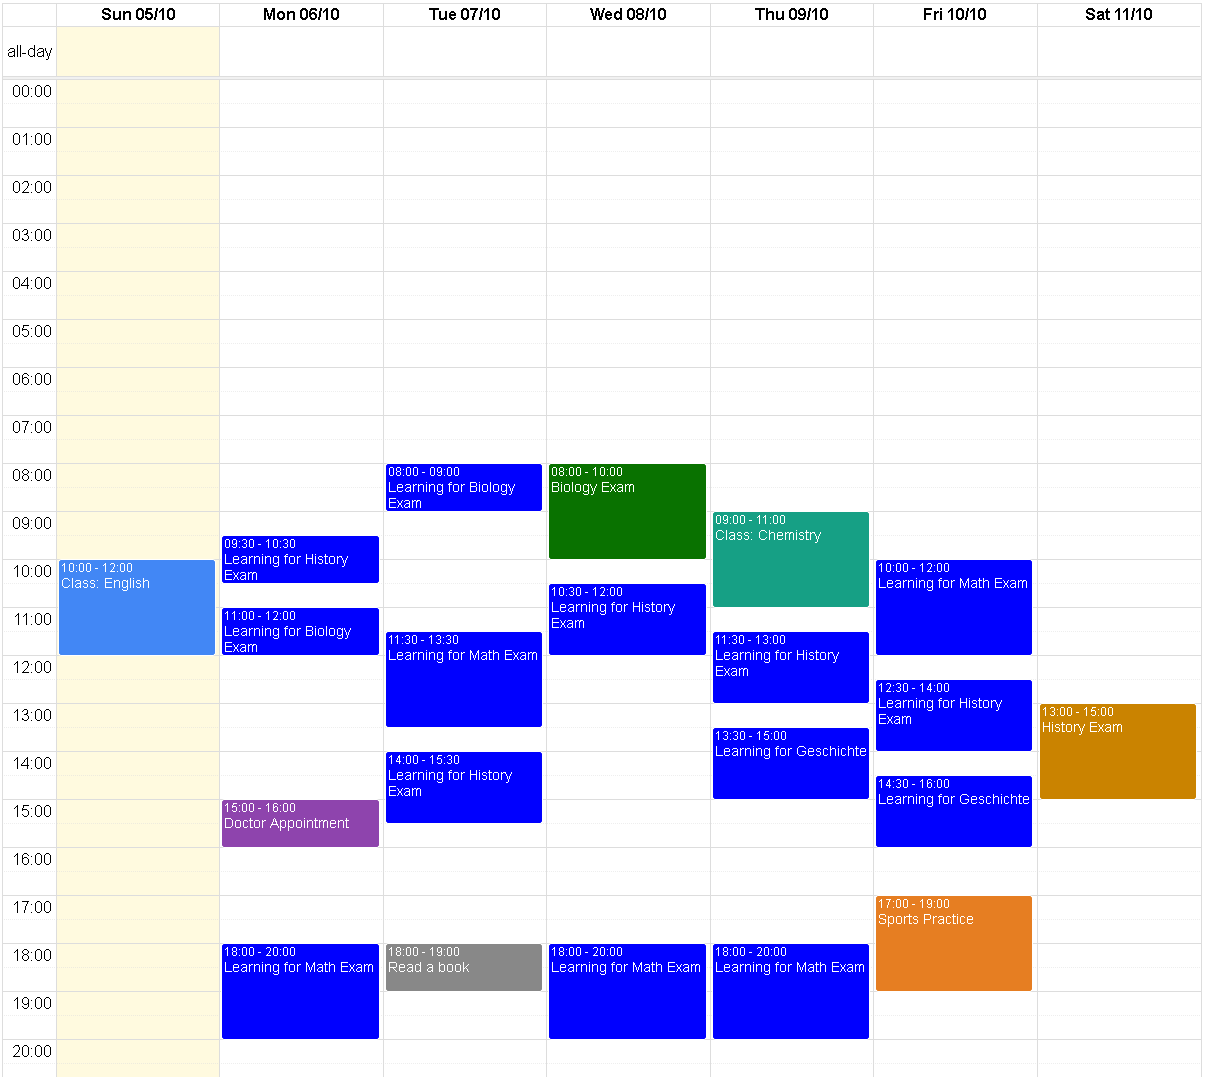
\includegraphics[width=\linewidth]{img/agenda.png}
    \caption{Beispiel einer Agenda, mit Lernblöcke von der LZA}
    \label{fig:placeholder}
\end{figure}
% ------------------------------ALGORITHMUS------------------------------
\subsection{Der Lernzeitalgorithmus}
Der Lernzeitalgorithmus (LZA) ist der Kern unserer Web-App. Er automatisiert die Planung der notwendigen Lernzeiten für die anstehenden Prüfungen eines Nutzers.

\subsubsection{Eingabeparameter und Planungsziel}

Der Lernzeitalgorithmus (LZA) verwendet globale Benutzereinstellungen sowie prüfungsspezifische Prioritätseinstellungen als Eingabeparameter, um eine optimale Lernplanung zu gewährleisten.

Das zentrale Planungsziel des LZA ist es, die definierten totale Lernstunden für jede Prüfung innerhalb des gültigen Lernfensters zu erreichen, während das tägliche Maximum und alle bestehenden Kalenderkonflikte des Nutzers strikt eingehalten werden.

\myparagraph{Globale Parameter}
Diese Einstellungen gelten für den gesamten Planungszeitraum:
\begin{itemize}
    \item \textbf{Lernen am Samstag}\\
    Definiert, ob der Algorithmus Lernblöcke an Samstagen planen darf.
    \item \textbf{Lernen am Sonntag}\\
    Definiert, ob der Algorithmus Lernblöcke an Sonntagen planen darf.
    \item \textbf{Bevorzugte Lernzeit}\\
    Die bevorzugte Uhrzeit am Tag, zu der die Platzierung von Lernblöcken primär angestrebt wird.
\end{itemize}

\myparagraph{Prüfungsspezifische Parameter (Pro Prioritätstufe)}
Diese Werte werden basierend auf der Priorität jeder Prüfung zugewiesen:
\begin{itemize}
    \item \textbf{Lernfenster}\\
    Die Anzahl der Tage rückwirkend ab dem Prüfungstermin, innerhalb derer Lernblöcke platziert werden sollen.
    \item \textbf{Tägliches Maximum}\\
    Die maximale Stundenzahl, die pro Tag für Prüfungen dieser Priorität geplant werden darf.
    \item \textbf{Total Lernstunden}\\
    Die gesamte Anzahl an Lernstunden, die für Prüfungen dieser Priorität absolviert werden muss.
\end{itemize}

\subsubsection{Ablauf und Planungsstrategie}
Der Algorithmus arbeitet iterativ und bearbeitet alle als Prüfung markierten Ereignisse in aufsteigender Reihenfolge ihrer Priorität. Eine niedrigere Prioritätsnummer kennzeichnet dabei eine höhere Wichtigkeit, um eine optimale Ressourcenverteilung zu gewährleisten.

\begin{enumerate}
    \item \textbf{Zyklische Neuberechnung der Anforderungen (Recycling)}:
    \begin{itemize}
        \item \textbf{Flexibilitätsbereinigung}: Alle vom System selbst geplanten, aber nicht gesperrten (gesperrt sind die Blöcke, die vom Nutzer bearbeitet worden sind) Lernblöcke für die aktuelle Prüfung werden gelöscht. Dies ermöglicht eine dynamische, optimale Neuplanung, falls sich die Rahmenbedingungen (z.B. neue Events, geänderte Prioritätseinstellungen) geändert haben.
        \item \textbf{Soll-Stunden-Ermittlung}: Die noch zu erbringende Lernzeit wird neu berechnet. Hierbei werden alle bereits absolvierten Stunden sowie Stunden, die durch manuelle oder vom Nutzer gesperrte Blöcke abgedeckt sind, von den Gesamtsollstunden abgezogen.
    \end{itemize}
    \item \textbf{Rückwärts-Iterative Planung}:
    \begin{itemize}
        \item Die Planungsstrategie ist eine Rückwärtsiteration: Sie beginnt beim Prüfungstermin und arbeitet sich tageweise bis zum aktuellen Datum vor. Dieses Vorgehen stellt sicher, dass die Lernblöcke mit höchster Dringlichkeit (die Tage, die am nächsten zur Prüfung liegen) zuerst belegt werden.
        \item An jedem Tag wird die maximale Lernzeit für diese spezifische Prüfung ermittelt. Diese ergibt sich aus der Differenz zwischen dem täglichen Maximum und den Stunden, die bereits an diesem Tag für die Prüfung geplant wurden. Dadurch wird das tägliche Zeitlimit zuverlässig eingehalten und eine Überlastung vermieden.
    \end{itemize}
    \item \textbf{Platzierung und strikte Konfliktvermeidung}:
    \begin{itemize}
        \item \textbf{Bevorzugter Slot}: Es wird primär versucht, einen Lernblock in der vom Nutzer festgelegten bevorzugten Lernzeit zu platzieren.
        \item \textbf{Konfliktprüfung}: Die Verfügbarkeit des Slots wird gegen alle Kalendereinträge des Nutzers für den aktuellen Tag geprüft. Dabei wird ein 30-minütiger Puffer vor und nach jedem bestehenden Ereignis (wie Sport oder Arzttermin) beachtet, um knappe Überlappungen und unnötigen Stress zu vermeiden.
        \item \textbf{Alternative Slots}: Falls die bevorzugte Zeit belegt ist, sucht ein dediziertes Modul den grössten verfügbaren, konfliktfreien Zeitabschnitt des Tages, um die Platzierung zu maximieren.
        \item \textbf{Echtzeit-Aktualisierung}: Nach der erfolgreichen Generierung und Speicherung eines Lernblocks wird dieser sofort zur Liste der aktuellen Kalenderereignisse hinzugefügt. Dieser Mechanismus ist entscheidend, um sicherzustellen, dass alle unmittelbar nachfolgenden Planungsversuche am selben Tag diesen neu erstellten Block als bereits belegt berücksichtigen und somit Überlappungen ausgeschlossen sind.
    \end{itemize}
    \item \textbf{Notfallplanung (Erweitertes Zeitfenster)}:
    \begin{itemize}
        \item Falls die Gesamtlernstunden nach der iterativen Planung im primären Lernfenster noch nicht erreicht wurden, aktiviert der Algorithmus eine Notfallsuche.
        \item Diese sucht nach verfügbaren Plätzen in einem erweiterten, sekundären Zeitfenster. Dieses Fenster erstreckt sich maximal bis zum 21. Tag vor der Prüfung.
        \item Die Regeln des täglichen Maximums und der Konfliktvermeidung bleiben auch in diesem Notfallmodus strikt erhalten.
    \end{itemize}
    \item \textbf{Ergebnisrückgabe und Zusammenfassung}:
    \begin{itemize}
        \item Nachdem alle Prüfungen bearbeitet wurden, gibt der Algorithmus eine detaillierte Zusammenfassung des Planungsvorgangs zurück.
        \item Diese Zusammenfassung informiert den Nutzer in einem Popup über die Gesamtzahl der hinzugefügten Lernblöcke und die Gesamtstunden, die erfolgreich geplant wurden.
        \item Zusätzlich wird für jede einzelne Prüfung der Planungsstatus (erfolgreich / nicht erfolgreich) und die geplante Stundenanzahl angezeigt.
    \end{itemize}
\end{enumerate}


% ------------------------------DAILY TIPS------------------------------
\subsection{Daily Tips}
Ein relativ wichtiges Feature unserer App sind die Daily Tips. Es sollte jeden Tag ein neuer Tipp an den Nutzer gezeigt werden auf der Startseite, entweder über die Kantonsschule oder allgemeine Lerntipps. Die einfachste Möglichkeit, dies zu implementieren, ist eine simple Modulo-Rechnung. 
\[
\text{Tipp des Tages} = (\text{Tag des Jahres}) \bmod (\text{Anzahl der Tipps})
\]

Somit wird an einem bestimmten Tag nur einen Tipp gezeigt und über das ganze Jahr sollten alle Tipps gezeigt werden (da wir sowieso weniger als 365 Tipps haben).


% ------------------------------NOTENORGANISATION------------------------------

\subsection{Notenorganisation}
In der Kantonsschule muss man immer wieder Prüfungen schreiben. Die Noten, die man erhält, sind dann wichtig für die Promotion in die nächste Stufe. Deswegen haben wir ein Feature, in dem man seine Noten pro Semester speichern kann. Jedes Semester hat schon die jeweiligen Fächer, die man dann in diesem Semester haben würde, geladen. Man kann natürlich immer noch Fächer löschen und hinzufügen. Man kann mit diesem Feature dann seine Durchschnitte pro Fach und Semester sehen. Ebenfalls kann man mit dem Notenrechner sehen, welche Note man in einem Fach brauchen würde, um einen bestimmten Schnitt in diesem Fach zu haben.

% ------------------------------LERNTIPPS/TIMER------------------------------



% References
\clearpage
%\addcontentsline{toc}{chapter}{Bibliography}
%\nocite{*}
%\printbibliography
\clearpage
\addcontentsline{toc}{chapter}{Literaturverzeichnis} % Changed from Bibliography/Quellen
\nocite{*}
\printbibliography[title={Literaturverzeichnis}]


\end{document}
